%%%%%%%%%%%%%%%%%%%%%%%%%%%%%%%%%%%%%%%%%%%%%%%%%%%%%%%%%%%%%%%%%%%%%%%%%%%%%%%%
% Template for USENIX papers.
%
% History:
%
% - TEMPLATE for Usenix papers, specifically to meet requirements of
%   USENIX '05. originally a template for producing IEEE-format
%   articles using LaTeX. written by Matthew Ward, CS Department,
%   Worcester Polytechnic Institute. adapted by David Beazley for his
%   excellent SWIG paper in Proceedings, Tcl 96. turned into a
%   smartass generic template by De Clarke, with thanks to both the
%   above pioneers. Use at your own risk. Complaints to /dev/null.
%   Make it two column with no page numbering, default is 10 point.
%
% - Munged by Fred Douglis <douglis@research.att.com> 10/97 to
%   separate the .sty file from the LaTeX source template, so that
%   people can more easily include the .sty file into an existing
%   document. Also changed to more closely follow the style guidelines
%   as represented by the Word sample file.
%
% - Note that since 2010, USENIX does not require endnotes. If you
%   want foot of page notes, don't include the endnotes package in the
%   usepackage command, below.
% - This version uses the latex2e styles, not the very ancient 2.09
%   stuff.
%
% - Updated July 2018: Text block size changed from 6.5" to 7"
%
% - Updated Dec 2018 for ATC'19:
%
%   * Revised text to pass HotCRP's auto-formatting check, with
%     hotcrp.settings.submission_form.body_font_size=10pt, and
%     hotcrp.settings.submission_form.line_height=12pt
%
%   * Switched from \endnote-s to \footnote-s to match Usenix's policy.
%
%   * \section* => \begin{abstract} ... \end{abstract}
%
%   * Make template self-contained in terms of bibtex entires, to allow
%     this file to be compiled. (And changing refs style to 'plain'.)
%
%   * Make template self-contained in terms of figures, to
%     allow this file to be compiled. 
%
%   * Added packages for hyperref, embedding fonts, and improving
%     appearance.
%   
%   * Removed outdated text.
%
%%%%%%%%%%%%%%%%%%%%%%%%%%%%%%%%%%%%%%%%%%%%%%%%%%%%%%%%%%%%%%%%%%%%%%%%%%%%%%%%

\documentclass[letterpaper,twocolumn,10pt]{article}
\usepackage{usenix}

% to be able to draw some self-contained figs
\usepackage{tikz}
\usepackage{amsmath}
\usepackage{nicefrac}
\usepackage{array,framed}
\usepackage{booktabs}
\usepackage{threeparttable}
\usepackage{multirow}
\usepackage{
  color,
  float,
  wrapfig,
  graphicx,
  caption,
}
\usepackage{setspace}
\usepackage{comment}
\usepackage{latexsym,fancyhdr}
\usepackage{url}
\usepackage{enumerate}
\usepackage{algpseudocode}
\usepackage{xparse}
\usepackage{xspace}
\usepackage{balance}
\usepackage{comment}
\usepackage{enumitem}
\usepackage{pifont}
\usepackage{stmaryrd}
\usepackage{centernot}
\usepackage{xcolor}
\usepackage{adjustbox}
\usepackage{tikz}
\usepackage{hyperref}
\usepackage{algorithm}



\usepackage{lang_sty/solidity}
\usepackage{lang_sty/llvm} 

\newcommand{\code}[1]{{\fontfamily{cmtt}\fontseries{m}\fontshape{n}\selectfont\small{#1}}}

\newcommand{\tool}{\textsc{GFL}}
\newcommand{\translator}{Emcc}
\newcommand{\wrapper}{Wrapper}
\newcommand{\runner}{Runner}
%-------------------------------------------------------------------------------
\begin{document}
%-------------------------------------------------------------------------------

%don't want date printed
\date{}

% make title bold and 14 pt font (Latex default is non-bold, 16 pt)
\title{\Large \bf {\tool}: Smart Contracts Fuzzing with GPU.}

\author{
{\rm Anonymous Author(s)}
} 

\maketitle

%-------------------------------------------------------------------------------
\begin{abstract}
%-------------------------------------------------------------------------------
Your abstract text goes here. Just a few facts. Whet our appetites.
Not more than 200 words, if possible, and preferably closer to 150.
\end{abstract}


\section{Introduction}

\noindent\textbf{Our contributions:}
\begin{itemize}
    \item ...
    \item ...
    \item ...
\end{itemize}   
\section{Background}

\subsection{Smart contract}

\subsection{CUDA}
\section{Design}
In this section, we not only describe the design of  {\tool} but also explain what challenges we need to solve for answering the reasons behind the design choices.  

\subsection{Overview}
Figure~\ref{fig:overlook} depicts the architecture of the {\tool}, which fuzzes a smart contract in GPU with thousands of threads.  
%
The process pipeline consisting of five steps. 
%
First, given an evm bytecode, {\translator} translates it into a functional equivalent LLVM assembly, where the Ethereum APIs (e.g. SHA3 and storage accesses) are implemented in device functions to avoid CPU.
%
Second, {\wrapper} creates a GPU kernel function in LLVM IR to wrap the contract code from {\translator}, for the parallel execution in GPU. The kernel function schedules graphic memory for thousands of GPU threads, making all threads can independently execute with different input. The wrapped LLVM assembly would be translated into a PTX executable as the final fuzzing target. 
%
In the third step, {\runner} generates various seeds to launch the PTX executable with thousands of threads at the same time. Apart from the extremely high throughput, {\runner} also designs incremental snapshots and coverage-based feedback to explore the smart contract deeper and faster since triggering a vulnerability in smart contracts usually requires several transactions\cite{}. 

\subsection{{\runner}: High Performance Fuzzing}
Throughput indicates the number of seeds can be tested by fuzzers in a time unit. The execution speed of the target program is the fundamental factor in fuzzing throughput\cite{fuzzan_atc}. 
Unfortunately, smart contract fuzzing suffers from serious throughput bottleneck, because smart contracts are designed to run on a virtual machine rather than a native environment. 
The blockchain virtual machine sacrifices its performance for the deterministic execution of smart contracts, in order to facilitate blockchain consensus protocols.
%
Under such execution layout, the existing smart contract fuzzers has to maintain a virtual machine and a blockchain database to test every single smart contract. 
%
Although running multiply fuzzers in parallel is one of effective and common-seen solution\cite{confuzzius_eurosp,echidna_issta ,afl,angora_sp,enfuzz_sec}, where all fuzzing threads share an identical global pool of seeds, the state-of-the-art tools still hit the upper bound due to the limited CPU cores number.
%
Therefore, in terms of fundamental aspect, the existing smart contract fuzzers cannot achieve high throughput (See \S~\ref{} for more details).
%

We believe the key of high performance fuzzing is testing a smart contract in as many parallel threads as possible without relying on blockchain virtual machines. 
%
Parallel fuzzing has no concurrency requirement, because all fuzzing threads can test the smart contract independently. The only synchronization event is used to wait for all fuzzing threads end. The more threads we can schedule, the higher throughput the fuzzer can achieve.
That is the reason why we choose to fuzz smart contracts on GPU. 
Different from CPU, GPU is full of stream processors, enabling running thousands of jobs in parallel. 
As far as we know, as one of the most powerful CPU, AMD Ryzen Threadripper PRO 5995WX (\$6,499) only has 64 cores, while a NVIDIA RTX3090 (\$999) can provide 10,496 CUDA cores\footnote{The prices come from the official vendor websites.}. 
The incredible computation power of GPU is attractive for parallel fuzzing as long as we can translate a smart contracts to GPU executable, i.e., PTX\cite{}. 
%
In CPU, we design {\runner} to launch a GPU device and fuzz the smart contracts with a batch of seeds. Once the GPU jobs are finished, {\runner} obtains the coverage information to feedback the seeds generations. 
%
In this section, we mainly elaborate the design and reasons of the fuzzing strategy that we choose. 
For example, to handle the transaction dependency, we enable smart contract running on GPU to create and restore snapshot for the storage variables (See \S~\ref{}). 
These strategies raise functional requirements to the smart contract and they can explain the design choices of the bytecode translation in \S~\ref{}.

% To benefit from feedback strategies and remain as high as possible throughput, there are two general approaches.
%
% One throughput improvement is boosting the execution of the fuzzing target. For example, AFL\cite{} enforces the fuzzing target initiate itself only once in the first fuzzing round and then clone its initiated process image to execute the remaining seeds.
%However, on the one hand, the redundant initiation is not the main computational overhead; on the other hand, a CPU can only provide limited threads ($<128$) for parallel execution.


\noindent \textbf{Parallel Execution on GPU}
Given a kernel function code, a GPU can schedule thousands of threads to execute a PTX code. 
%
Each thread copies the PTX code in its code segment and then extracts different input from CPU to produce different output in parallel. 
To be specific, each thread is labeled with an auto-increment ID (i.e., thread ID) and run in a specific CUDA core. 
Since the global memory is visible for all threads, we allocate a sequential memory to maintain all thread input. We pad every seed to 128 bytes so that each thread can compute the address offset of its input using its thread ID. For example, $calldata = p + threadId * 128$, where $calldata$ points to a thread seed. 
Considering {\tool} is a coverage-based fuzzer, the coverage information recorded in the bitmap should be the output of the executed smart contract. 
We adopt similar approach to map the bitmap to global memory taking thread ID as the index. 
In \S~\ref{} we will explain the details of bitmap instrumentation. 
%
To make each thread run independently, we ensure each smart contract code to run in a local context. Hence, threads do not have to wait each other.
%
% To make each thread run efficiently, we should create a coalescing memory and avoid strike access.
% Figure~\ref{} shows the data structure of memory layout.

% an example of data layout
% threadIdx = grid.x * block.x * thread.idx

% transaction size: why not use compact mode. 
% Our memory model is strided
% https://developer.nvidia.com/blog/how-access-global-memory-efficiently-cuda-c-kernels/
% aligned memory.

\noindent \textbf{Fuzzing with Transaction Dependency}
\label{design:snapshot}
Smart contract is a stateful program, which maintain states variables in its storage. Since the state variables can be part of the path constraints, some branches can be explored by fuzzers when smart contract is set as a specific state. 
%
As the example shown in Figure~\ref{}, the vulnerability in function $vul()$ can only be triggered when the state variable named $flag$ is set to $``poc"$ via executing $set(``poc")$ first. 
%
To explore more branches, existing fuzzing tools decide to generate transaction sequences based on the transaction dependency\cite{confuzzie, echidna}. 
To be specific, they fix one transaction first and combined it with a following transaction to generate a seed. However, they may execute duplicated transactions when fuzzing with sequence-based seeds. These redundant execution wastes the computational resource, resulting in low throughput. 
%
% Not to mention the challenge to recognize transaction sequences. 
% The existing fuzzers on smart contract find ideal transaction sequences based on the data flow of storage variables, which is still a open question. Storage is a key-value structure. The key of storage variables may be a hash value which is challenging to recognize 
% However, these approaches did not label which states are interesting but continue to find transactions based on the data flow graph. 
%
In order to fulfill the transaction dependency, we design a snapshot strategy to record interesting states of the smart contract. An interesting seed means new coverage is recorded in the bitmap. A program state executed after an interesting seed is an interesting state. 
Whenever we found an interesting state, we create a storage snapshot representing the program state. 
The created state snapshots are maintain in the CPU end. 
In the next fuzzing iteration, {\tool} can restore a selected snapshot to further test the smart contract.
By switching snapshots, {\tool} can allocate more energy on the interesting state to facilitate the transaction dependency without executing duplicated transactions. Moreover, we can initiate the storage with real-world data to test on-chain smart contract in any stages, hence the found payload can be still effective on mainnet. 
%
Since snapshot switches require additional data exchange between CPU and GPU, we must reduce the consumption of graphics memory, enabling {\tool} to conquer the memory latency between CPU and GPU, which is the main bottleneck in CUDA programming. 
To this end, we further design a Redirect-On-Write storage (See \S~\ref{}) to make the snapshot create and reload operations light and fast.


\noindent \textbf{Encoding States Changes into Bitmap}
Traditional coverage-based fuzzing can only recognize control flow. For example, AFL uses a tuple $(id_{src}, id_{dst}$ to recorded an explored control flow, i.e., an edge from one basic block to another one. Whenever a basic block is executed, AFL increases one bitmap byte in the index of $(id_{src} * 2) \oplus id_{dst}$. 
% TODO
To record the side effect of states changes, we extend the bitmap as follow $state_0 \oplus ... \oplus state_n \oplus (id_{src} * 2) \oplus id_{dst}$, where $state_i$ indicates the storage states. 
Whenever the storage is updated, the bitmap can add one bit to reflect such change. 
As aforementioned before, the example in Figure~\ref{} has transaction dependency.  



\begin{figure}[t]
\begin{algorithm}[H]
\caption{Storing a storage state into the ROW snapshot.}
\label{algo:row_sstore}
\begin{algorithmic}[1]
    \Require $key$, the storage index; $val$, the storage state
    \State $Src \gets initial storage states$
    \State $Snap \gets the storage states snapshot$
    \If{$key \in \{s.key \mid s \in Snap\}$} 
        \State $Snap[key].val = val$
        \State \Return
    \EndIf
\end{algorithmic}
\end{algorithm}
\end{figure}


\begin{figure}[t]
\centerline{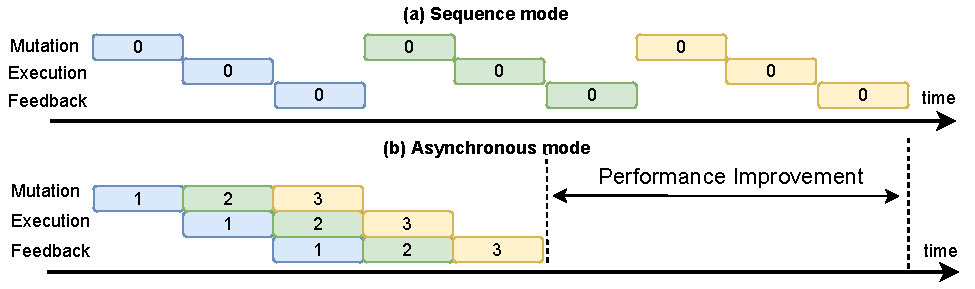
\includegraphics[width=0.5\textwidth]{images/GFL-async_cpy.drawio.pdf}}
\caption{Fuzzing Timelines}
\vspace{-0.1in}
\label{fig:async_cpy}
\end{figure}

\noindent \textbf{Asynchronous Fuzzing}
\label{design:asynchronous}
As far as we know, all traditional coverage-based fuzzers are implemented on CPU in synchronous mode. Each fuzzing iteration consists of three sequence steps, such as seed mutation, target program execution, and coverage bitmap analysis. 
On the one hand, target program execution cannot run until the seed variant is prepared by the fuzzers. 
On the other hand, fuzzers have to wait the target program execution ends and then can analyze the coverage information for next round fuzzing iteration. 
To enhance the throughput performance, {\tool} aims to reduce the time intervals between these three steps.
Since GPU and CPU are two independent devices, {\runner} can submit fuzzing jobs to GPU and then immediately back to CPU to mutate seeds and analyze the coverage information without waiting the GPU. 
In Figure~\ref{}, we show the timelines for sequence mode (a) and asynchronous mode (b) in a three times fuzzing. 
{\tool} creates three stream pipeline to handle the three group of fuzzing jobs in asynchronous mode. 
The jobs in the same stream are highlighted in the same color. 
In the first time slot, we mutate seed on CPU only. In the next slot, we can run stream \#1 and \#2 together, which launches GPU and mutate seeds, respectively. At last, {\tool} can finish the fuzzing work in five slots, which is less than the traditional methodology (nine slots).

Moreover, asynchronous design enables {\tool} to reduce the overhead of memory latency. \cite{} analyzes the CUDA overhead and finds transferring data between CPU and GPU is time-consuming. {\tool} can invoke another streams when the memory bus of GPU is stuck to one stream job. 


    
\subsection{{\translator}: Functional Equivalent Program Generation}
\label{design:translator}
We rewrite the target smart contracts for various purposes, such as 1) generating PTX code to run on GPU, 2) inserting sanitizers to capture crashes, 3) instrumentation for obtain coverage information necessary. 
To rewrite the code more flexible and precise, we build an IR-based framework based on decide to LLVM intermediate representation.
%
Broadly speaking, there are two approaches to obtain the llvm assembly of an Ethereum smart contract: 1) Source code compilation by converting Solidity to C++ first and generate IR from clang\cite{}; 2) Binary translation from an EVM bytecode. 
We choose to use binary translation because blockchain public every smart contract and encourage nodes to execute and verify them, for satisfying consensus protocol. {\tool} can test the real-world smart contract as it is deployed. 
We exclude the source code approach because Solidity does not support LLVM and the existing Solidity to C++ parser has serious compatibility issues as Solidity grammar updates quite often. Moreover, even there exist available source code tools, developers have to recompile the target with flags, which may be opaque for the testing. 


\noindent \textbf{devirualization}
%basic block
We decide to obtain the intermediate representation of the given smart contract to generate a PTX program. 
EVM bytecode is a sequential of stack-based opcodes, which can be lifted to an registers-based LLVM assembly via devirualization and mem2reg\cite{}. 
We allocate an LLVM array as the EVM stack and thus EVM opcodes can be represented as memory accesses. 

\noindent \textbf{jumps recovery}
All EVM jumps such as \code{\%JUMP} and \code{\%JUMPI} are indirect jumps, which take the stack top as the jump destination. 
To recover the control flow of the smart contract bytecode, we lift EVM jumps as table jumps. 
Since an EVM jump must go to a basic block where the first opcode is \code{JUMPDEST}, we can recover the jump table by 

A table jump decides its jump destination until the GPU runtime when it loads the stack top from the emulated stack and then query

% We allocate an LLVM array as the EVM stack (denoted as \code{\%stk[]}) and thus EVM opcodes can be represented as memory accesses. We use an LLVM register named \code{\%sp} represented as the index of \code{\%stk[]}, which maintains the current stack height. For example, we can load the stack top using \code{\%stk[\%sp]}. By adjusting \code{\%sp}, we can push and pop data from the evm stack. 
% In general, \code{\%stk[]} consists of 1,024 256-bits elements, following the semantic setting of EVM.


\noindent \textbf{Simulating Environment Opcodes}
Some EVM opcodes are external interfaces of blockchain environment.
On the one hand, smart contracts can interactive with blockchain environment with specific opcodes, such as TIMESTAMP for loading the timestamp and NUMBER for obtaining the current block height. Although blockchain client provided restful APIs that we can import to lift the environment opcodes, it requires GPU to wait data from CPU, which sharply decrease the {\tool} throughput.
%
On the other hand, smart contract is big endianness rather than the little endianness used in GPU architecture. 
To make smart contract can run in GPU, we need to simulate the environment opcodes inside GPU and convert the endianness. 
For each kind of environment opcodes, we create a device function:
\begin{itemize}
    \item `get' approaches: return constants
    \item hash function: implement the keccak256  method;
    \item storage accesses: read and store data from a ROW snapshot (See \S~\ref{});
    \item load input data: load data from the CPU in little endianness.
    \item memory operations: read and store data from \code{\%mem} in little endianness.
\end{itemize}

Note that, each thread only access the local memory to avoid threads synchronization.

\noindent\textbf{Storage}
{\tool} can perform snapshot reload and creation operations fast and light. This design is based on our observation that a transaction usually only modified specific storage variables. Therefore, the states of a smart contract share parts the same content. That is the reason why we create a snapshot-based storage. 
Given an initial storage, we schedule thousands GPU threads to test the state. We store the initial storage in global memory as the source volume, broadcasting its content to every thread. Every thread create a ROW snapshot in its local memory to avoid synchronization. If the seed is interesting, we export the storage snapshot to CPU and combine it with the source volume to build a full storage snapshot.   
%
We first initiate a source volume as the initial storage of the smart contract, and then create a Redirect-on-write (ROW) snapshot for each fuzzing thread. The snapshot maintains all storage states of the given smart contract, enabling each GPU thread to use minor memory to record the states changes. 
Whenever the smart contract stores a state into its storage (i.e., \code{SSTORE}), we save the state in the snapshot. As for the storage loading activities (i.e., \code{SLOAD}), we first enquiry from the snapshot and then the source volume. 
If the seed is interesting, we export the storage snapshot from GPU to CPU. 
We can reload a full storage by combined the exported snapshot and the source volume together. The full storage will become the initial storage in next fuzzing iteration.
\section{Implementation Details}

In order to evaluate the impact of our design choices, we implement a prototype for {\tool} using approximately 6,000 lines C++ code.
The prototype implementation will be open source after this paper being accepted.

% \subsection{{\wrapper}}

As smart contracts are designed for sequential execution, it is challenging to enforce the lifted IR to handle multi-thread execution scheme. 
To this end, we extend the generated IR to make sure it can be translated into retargetable code.
Specifically, we isolate the memory layout of each GPU thread, such as calldata, stack, memory and storage.
Each thread can access the same address size of GPU memory but with different offset. Once the GPU threads are launched together, they use the same code code but accept different input to get different execution results. In the end, the fuzzer can combined all threads results to decide what seeds should be tested in next round.

As the GPU entry, we create a kernel function named \code{@main} to acquire the input and execution smart contract with a sequence of transactions. 
As there will be thousands of threads running on GPU together, we need to isolate the execution context of each thread. 
Figure~\ref{} shows the data layout of the GPU smart contract. $ninput$ and $nbitmap$ are two large consistent memory.
We allocate a graphic memory as the bitmap for all threads. Each thread is designed to record the coverage information in its bitmap only, i.e., $nbitmap[id*size\to id*size+size]$. 
Each thread calculate its thread ID via $id = blockIdx.x * blockDim.x + threadIdx.x$. Then it can load its input from the graphic memory, i.e., $ninput[id*width\to id*width+width]$. $width$ is the input size of each thread. 
Figure~\ref{} indicates the data structure of the thread input, including several transaction data. Each transaction data include the callvalue, calldatasize and calldata. We parse the transaction data to invoke the smart contract, i.e., \code{@contract}. To analyze the transaction sequences effects, we call \code{@contracts} in sequence several times. 
In \code{@main}, we calculate the memory offset for each thread to access its bitmap and input.
Therefore, whenever a thread is scheduled, it can only write its local memory. In other words, our GPU jobs are unnecessary to ensure synchronization, which means threads can run faster as they do not have to wait for peer threads. 

% ----------------+----+----------+
%   calldatasize1 | tx1| ... txn  | ...  
% ----------------+----+----------+
% <----------------- thread1 -----><-------- threadn ---->

% ----------------+----------+----------+
%  bitmap1        | bitmap2  | ...  
% ----------------+----------+----------+
% <-- thread1 --->...........<-----threadn ---->


\subsection{{\translator}}

\subsubsection{Basic Blocks Construction}
EVM bytecode is a sequence of opcodes which are organized in several basic blocks connecting in control flow.
Each EVM basic block must follow the below two rules: 1) starts with \texttt{JUMPDEST}; 2)ends with a terminator such as jump (\texttt{JUMP} and \texttt{JUMPI}) and halt (\texttt{RETURN}, \texttt{STOP}, \texttt{REVERT} and \texttt{SELFDESTRUCT}).
We label each basic block with the program counter of its head opcode. 


\subsubsection{Devirtualization}
 but also declare several local data for each thread, such as EVM memory, EVM stack and storage. 
We use a device function named \code{@contract()} to include the smart contract. \code{@contract} is the main entry of the smart contract, which accepts transaction data and runs smart contract code on the local stack, memory and storage. At last, each thread update its bitmap. 

We allocate an LLVM array as EVM stack named \code{@custk} and a stack pointer named \code{@sp}. For each basic block, we extract the used operands but defined outside. For example, \code{@custk[@sp--]} indicates popping an element from stack. 
Since all jumps in EVM bytecode are indirect. We additionally allocate a variable named \code{@pc}. When we meet a jump like \code{JUMP} or \code{JUMPI}, we set \code{@pc} as the value of stack top. And then perform a table jump, like \code{table jump \%pc, []}, where the tables indicate the entries of all basic blocks.


\subsubsection{Environment Opcodes}
We create native functions for lifting the environment Opcodes. To be specific, we implement these native functions in C++ source code and then compile into library code in LLVM assembly. We elaborate the linkage setting to make the lifted bytecode can link with the library code. 

For contract calls, we lift them to functions calls where each function indicates the logic of a bytecode. 
For \code{CALLDATALOAD}, we read data from the GPU memory and return in little-endianness. 
For \code{TIMESTAMP} and other get methods, we return constants for simulation. 
Base on the above designs, we can ensure the smart contract on GPU has consistent execution results as it run on CPU, in terms of basic functions.

\subsubsection{Use a Incremental Snapshot}

Storage maintain the persistent data of a smart contract, which may result in transaction dependency.
We simulate a storage inside the GPU for each thread. Since all threads start from the same storage snapshot, we can create snapshot for each thread, for reducing redundant memory. 
For example, we create a global storage as initial data and then allocate a local storage for each thread. 
Each local storage is the incremental snapshot of the global storage. Therefore, we can perform ROW storage accesses.
We store new storage data into the local thread. When loading storage data, we first check whether the local storage exists the data, if no exist, we the search the global storage. If no data is found, we return the default value zero following the EVM semantic. 

\subsubsection{Schedule Incremental Snapshots}



\begin{figure}[t]
\begin{algorithm}[H]
\caption{Loading a storage state from the ROW snapshot.}
\label{algo:row_sload}
\begin{algorithmic}[1]
    \Require $key$, the storage index
    \State $Src \gets \texttt{initial storage states}$
    \State $Snap \gets \texttt{the storage states snapshot}$
    \If{$key \in \{s.key \mid s \in Snap\}$} 
        \State \Return $Snap[key].val$
    \Else
        \If{$key \in \{s.key \mid s \in Src\}$}    
            \State \Return $Src[key].val$
        \Else
            \State \Return 0
        \EndIf
    \EndIf
    % \For{ each: \texttt{$s \in Snap$}}
    %     \If{$s.key = key$} 
    %         \State \Return $s.val$
    %     \EndIf
    % \EndFor
\end{algorithmic}
\end{algorithm}
\end{figure}


\subsection{{\runner}}

\subsubsection{Asynchronous Fuzzing}
The initiation and execution phase of PTX is naturally two parts. We can explicitly initiate the kernel function one time and launch it with multiply threads in any times. It would help us to reduce the overhead because of initiation\cite{cudaoverhead}.

Once we got the CUDA context, we upload the initial storage data to GPU to bind the global storage. Then we prepare perform asynchronous Data Transfer between CPU and GPU. 

In each stream, the index of launched threads starts from zero. To enable threads in all streams can accept multiply input and report all output, we split the input for each stream.
Each stream uses an offset.
For example, the threads $i$ in stream $n$ can access $calldata = offset + i * size$, $snap[offset + i]$.



\subsubsection{Snapshot schedule}
We create a queue to maintain all snapshot. To reload the snapshot, we first get the symbol of the global variable of the source storage used in the GPU thread. Second, we query the memory table to find out the GPU address of the symbol. At last, we can copy the expect storage from CPU to the GPU graphic to initiate the source snapshot. The source snapshot stays in the constant memory, thus it is visible for all GPU threads. 

Each snapshot only used in local memory to make all threads run independently. To export the storage, we also create a shared memory between CPU and GPU for export the expect storage snapshot. The shared memory have the same size of the storage snapshot. Due to the limited size of the global memory, we cannot declare all storage snapshot in the global memory, but random select one thread to export its snapshot if it executed with a interesting seed.
% 为什么不直接在global memory声明storage,这样还能全数倒出snapshot
% => 考虑global memory和local memory的大小,seeds和bitmap等都需要写入到global memory

\subsubsection{Seed Mutation}
Each smart contract function has an explicit definition recorded in the ABI, which is public to blockchain along with the bytecode.
For each function argument, we mutate it based on its type. 
\section{Evaluation}

\subsection{Experiment Environment}
All experiments were performed on a server running Ubuntu 18.04 LTS with dual Intel Xeon Gold 6226R CPUs, 512 GB RAM and one Nvidia RTX3090-24G.
The CUDA library version is v11.3.
%
We ask GPU to run 4,096 streaming multiprocessors (SM). Each SM schedules 32 CUDA cores. 
%
For each smart contract, we test XXX minutes. The total experiment costs XXX CPU days. 

\subsection{Correctness}
\label{rq:correctness}

\subsubsection{Motivation}
We need to ensure the bytecode transaction is function equivalent. To this end, we collect POC from the Ethereum community and replay on CPU and GPU to compare the storage contents. 
% evaluate the sanitizers as well.
\subsubsection{Approach}

\subsubsection{Results}


\subsection{Throughput}
\label{rq:throughput}

\subsubsection{Motivation}
Throughput is the fundamental factor of fuzzing tools.

\subsubsection{Approach}

\subsubsection{Results}
\input{sec-discussion}
\section{Related Work}

\subsection{Coverage-based Fuzzing}
%hardware Intel-PT, RISC-V CRS
%binary Pin
%IR based

\subsection{Parallel Fuzzing}
% single machine
% cluster

\subsection{Code Vectorization}
%SIMD

\section{Conclusion}
We design and develop {\tool}, a novel fuzzer that converts EVM contracts to PTX contracts to test on SIMD GPU and provides an snapshot strategies to the smart contract in different stages. 
%
We conduct extensive experiments to evaluate {\tool}, and the experimental results show that the throughput of {\tool} can reach XXX, which exceeds all existing tools XX.



%-------------------------------------------------------------------------------
\bibliographystyle{plain}
\bibliography{bib}

%%%%%%%%%%%%%%%%%%%%%%%%%%%%%%%%%%%%%%%%%%%%%%%%%%%%%%%%%%%%%%%%%%%%%%%%%%%%%%%%
\end{document}
%%%%%%%%%%%%%%%%%%%%%%%%%%%%%%%%%%%%%%%%%%%%%%%%%%%%%%%%%%%%%%%%%%%%%%%%%%%%%%%%

%%  LocalWords:  endnotes includegraphics fread ptr nobj noindent
%%  LocalWords:  pdflatex acks